\lecture{Estimador de tempo de símbolo}{lec_carrier}

\begin{frame}
	\begin{block}{\centering\large\bfseries Parte 7}
		\centering\large\insertpart
	\end{block}
\end{frame}

\section{Introdução}
\begin{frame}[t]
	\frametitle{Introdução}
	
	\begin{itemize}
        \item Em métodos \textit{clock-aided}, o transmissor envia o relógio do modulador separado do \textit{stream} de dados. Dizemos então que este método de transmissão é \emph{síncrono}.
        \item No entanto, para diversas aplicações, a transmissão de um relógio separado seria ineficiente, uma vez que isso exigiria recursos adicionais (largura de banda, potência, etc...).
        \item Como alternativa, faz-se necessário implementar um circuito adicional que recupere o tempo de símbolo no demodulador.
        \item O requerimento fundamental do estimador de relógio é que instante de símbolo seja recuperado, mesmo que imperfeitamente. Em outras palavras, a partir do envelope complexo do sinal recebido, o demodulador precisa saber qual é o instante de tempo no qual o \(k\)-ésimo símbolo transmitido inicia.
    \end{itemize}
\end{frame}

\section{Tipos de recuperação de relógio}
\begin{frame}[t]
	\frametitle{Tipos de recuperação de relógio}
    \begin{figure}
        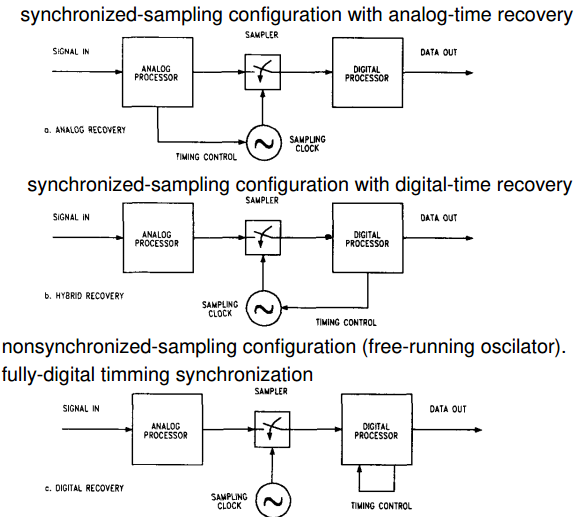
\includegraphics[scale=.3]{figs/tipos_de_sinc_de_relogio.png}
    \end{figure}
    \begin{itemize}
        \item A implementação de um detector completamente digital só é possível com a adoção do método de transmissão assíncrono.
    \end{itemize}
\end{frame}

\begin{frame}[t]
    \frametitle{Método de recuperação de relógio completamente digital}
    \begin{itemize}[<+->]
        \item No caso do método de recuperação de relógio completamente digital, como recuperar o relógio?
        \item \emph{Resposta}: através da \emph{interpolação} do sinal discretizado.
        \item Como a correção do instante de símbolo é implementada?
        \item \emph{Resposta}: utiliza-se três módulos funcionais que integram o chamado sincronizador de relógio \cite{abrantes2010recuperaccao}:
            \begin{itemize}
                \item<.-> Interpolador: responsável por corrigir o instante de amostragem do sinal discreto.
                \item Controlador: utiliza o sinal de erro proveniente do estimador para gerar a parte inteira e fracionária do novo instante de símbolo.
                \item Estimador do atraso de símbolo: gera um sinal de erro em relação à estimativa do atraso de símbolo. É aqui onde a estimação propriamente dita acontece.
            \end{itemize}
    \end{itemize}
\end{frame}

\section{Técnicas de estimação de relógio}
\begin{frame}[t]
	\frametitle{Técnicas de estimação de relógio}
    \begin{itemize}
        \item Dentre os métodos re recuperação de temporização assíncronos (\textit{non-clock-aided}), estes ainda podem ser classificados como segue
    \end{itemize}
    \begin{figure}
        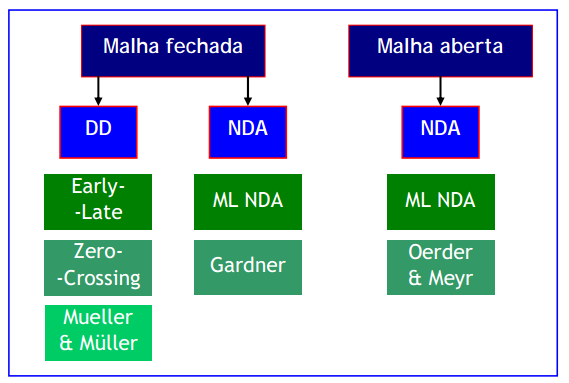
\includegraphics[scale=.45]{figs/tecnicas_estimacao.png}
    \end{figure}
\end{frame}

\section{Controlador}
\begin{frame}[t]
	\frametitle{Controlador}
    \begin{itemize}
        \item Precisamos, a partir das amostras vindas do oscilador local operando em \textit{free-running} e do sinal de erro proveniente do estimador, obter novas amostras.
    \end{itemize}
	\begin{figure}
        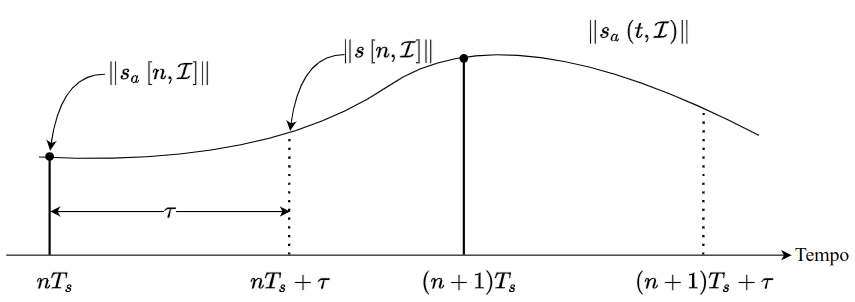
\includegraphics[scale=.35]{figs/sync_time.png}
    \end{figure}
\end{frame}

\begin{frame}[t]{Controlador}
    \begin{itemize}
        \item \begin{IEEEeqnarray}{rCl}
            \label{eq:tau_k}
            \hat{\tau}_k & = & \hat{\tau}_{k-1} + \gamma_\tau e_{\tau} \left[k\right]
          \end{IEEEeqnarray}
          \begin{itemize}
            \item \(\gamma_\tau\): passo de aprendizagem.
            \item \(e_{\tau} \left[k\right]\): Sinal de erro proveniente do estimador de atraso de símbolo.
          \end{itemize}
        \item Os instantes de interpolação podem ser definidos como
        \begin{IEEEeqnarray}{rCl}
          \label{eq:t_n+1}
          t_{n+1} & = & t_n + T_s + \frac{\gamma_\tau}{N}\dot{e}_\tau \left[n\right],
        \end{IEEEeqnarray}
        em que $t_n$ indica o instante de amostragem do sinal $\dot{r} \left[n\right] \triangleq r \left(t_n\right)$, sendo $r \left(t\right)$ o envelope complexo contínuo do sinal recebido.
    \end{itemize}
\end{frame}

\begin{frame}[t]
    \frametitle{Controlador}

    \begin{itemize}
        \item Note que, se normalizarmos $t_n$ por $T_s$, obteremos uma parte inteira, $l_n$, e uma parte fracionária, $0\leq \mu_n < 1$. Matematicamente, tem-se
        \begin{IEEEeqnarray}{rCl}
          \label{eq:t_n}
          t_n & = & T_s \left( l_n + \mu_n \right).
        \end{IEEEeqnarray}
        \item Tomando as partes inteiras e fracionárias de ambos os lados, tem-se
        \begin{IEEEeqnarray}{rCl}
            \label{eq:l_n+1}
            l_{n+1} & = & l_n + 1 +  \floor*{\mu_n + \frac{\gamma_\tau}{NT_s}\dot{e}_\tau \left[n\right]}
        \end{IEEEeqnarray}
        e
        \begin{IEEEeqnarray}{rCl}
            \label{eq:mu_n+1}
            \mu_{n+1} & = & \mathrm{frac}\left(\mu_n + \frac{\gamma_\tau}{NT_s}\dot{e}_\tau \left[n\right]\right),
        \end{IEEEeqnarray}
        em que $\mathrm{frac}\left(x\right) \triangleq x - \floor*{x}$ indica a parte fracionária de $x$.
    \end{itemize}

\end{frame}

\begin{frame}[t]
	\frametitle{Controlador}
	\begin{figure}
        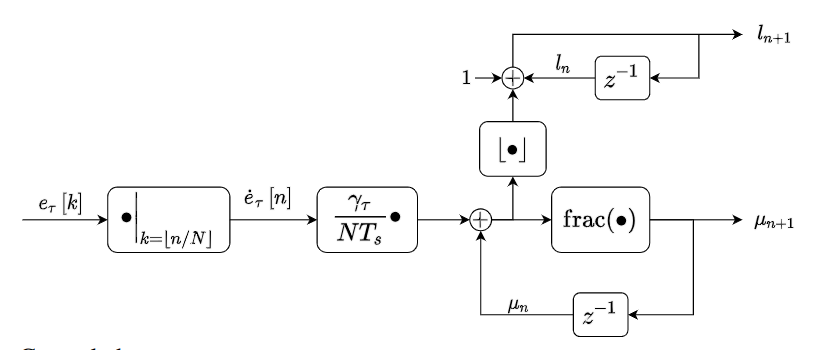
\includegraphics[scale=.4]{figs/interpolator.png}
    \end{figure}
\end{frame}

\begin{frame}[t]
	\frametitle{Exemplo de sincronismo de tempo}
	\begin{figure}
        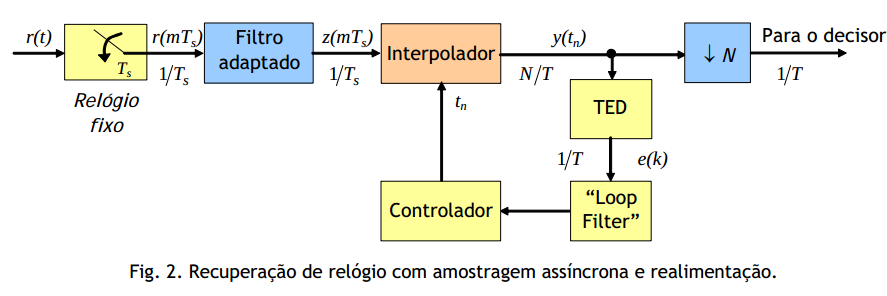
\includegraphics[scale=.4]{figs/time_synch.png}
    \end{figure}
\end{frame}

\begin{frame}[t]
	\frametitle{Exemplo de sincronismo de tempo}
	\begin{figure}
        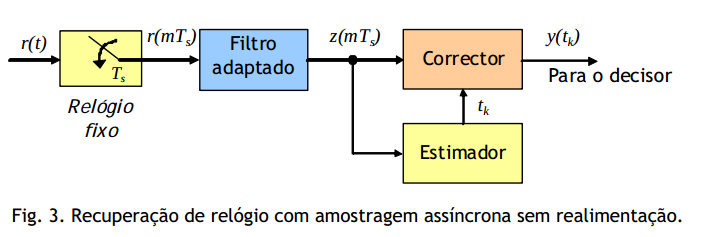
\includegraphics[scale=.4]{figs/time_synch2.png}
    \end{figure}
\end{frame}